\documentclass[a4paper,12pt]{article}
\usepackage[utf8]{inputenc}
\usepackage{polski}                             
\usepackage{fontenc}                            
\usepackage{graphicx}                            
\usepackage{textcomp}                            
\usepackage{enumerate}
\usepackage{indentfirst}
\usepackage{hyperref}
\usepackage{authblk}
\usepackage{url}
\usepackage{float}
\usepackage[a4paper, left=2 cm, right=2 cm, top=3cm, bottom=3cm,]{geometry}
\hypersetup{colorlinks=true, linkcolor=black, urlcolor=black}
\usepackage{secdot}
\title{\textbf{FAQ - Często zadawane pytania przez przyszłych i początkujących radioamatorów}}
\author{Fundacja Hackerspace Kraków
oraz klub SP9KGP\\
Licencja: CC-BY-NC-SA\\
\vspace{1ex}
Autorzy:\\
Krzysztof SQ8RK\\
Paweł SQ9PID\\
Szymon SQ9ZAQ\\
Kuba\\
Jacek\\
Tadek SP9TED\\
Wojciech SQ9PBS\\
Wiktor SQ9WTF\\
Marcin SQ9ONH\\
Arek SQ3PMK\\
Marcin SP5XMI\\
Tomek SP7Q}                             


\begin{document}
\maketitle

\newpage
%\tableofcontents
\newpage

\section{Wstęp}
Pasmo, modulacja, propagacja… Te dziwne słowa usłyszane od znajomych sprawiły, że zaczęliśmy szukać informacji o radiu i krótkofalarstwie. Pojawiło się wiele pytań, którymi zadręczaliśmy kolegów. Pierwsze nasłuchy, nauka do egzaminu krótkofalarskiego czy przygotowania do pierwszego „QSO” dołożyły do tej listy kilkanaście kolejnych pozycji. Postanowiliśmy je spisać, zarówno te „trywialne” jak i te bardziej szczegółowe, po czym poprosiliśmy bardziej doświadczonych kolegów o zredagowanie odpowiedzi, które można by zamieścić w „FAQ”. Tak oto powstał niniejszy dokument. Nie wyczerpuje on tematu, ale wierzymy że każdy początkujący znajdzie tutaj interesujące go pytania i zrozumiałe odpowiedzi. 

Życzymy przyjemnej lektury i… do usłyszenia na pasmach! 73!

\section{Co tak właściwie daje nam krótkofalarstwo i po co ono jest?}
Według definicji regulaminu radiokomunikacyjnego\footnote{\url{www.gov.pl/web/instytut-lacznosci/regulamin-radiokomunikacyjny-itu}}, to ,,służba radiokomunikacyjna mająca na celu samokształcenie,
wzajemne komunikowanie się i badania techniczne prowadzone przez amatorów, tj. przez odpowiednio upoważnione osoby interesujące się techniką radiową wyłącznie z pobudek osobistych,
a nie w celu zarobkowym.''. Jak sama nazwa mówi - daje to satysfakcję z tego, że się porozmawia z kimś ciekawym - tak samo można mieć satysfakcje z skonstruowania sprzętu lub zrobienia dalekiej, czy rzadkiej łączności.

\section{Jaki sprzęt jest potrzebny na początek zabawy?}
Na początek  “starter kit-em”, który pozwala na lokalną łączność na fonii, jest mniej więcej coś takiego:
\begin{itemize}
 \item chińskie radio ręczne, na przykład Quansheng UV-K6 lub w przypadku większego budżetu coś producentów Yaesu, Icom czy Kenwood. 
 \item przejściówka na najczęściej używane złącze UC-1 (zwane też M lub UHF)
 \item antena własnej produkcji (np. prosty dipol półfalowy) lub kupna (np. typu 2x5/8 \(\lambda\))
\end{itemize}
\section{Jakie częstotliwości radiowe obejmują określone kategorie pozwoleń?}
\begin{itemize}
\item Dla kategorii 1 - wszystkie, to znaczy - 160 m (1,8 MHz), 80 m (3,5 MHz), 60 m (5 MHz), 40 m (7 MHz), 30 m (10 MHz), 20 m (14 MHz), 17 m (18 MHz), 15 m (21 MHz), 12 m (24 MHz), 10 m (28 MHz), 6 m (50 MHz), 4 m (70 MHz), 2 m (144 MHz), 70 cm (430 MHz), 23 cm (1.2 GHz), 13 cm (2.3 GHz) i wyższe (pasma mikrofalowe). 
\item Dla kategorii 3 są to pasma 160 m, 80 m, 40 m, 20 m, 15 m, 10 m, 2 m, 70 cm i 3 cm (10GHz)\footnote{\url{http://isap.sejm.gov.pl/isap.nsf/download.xsp/WDU20150000099/O/D20150099.pdf}}.\end{itemize}


\section{Co to w ogóle jest to „pasmo”?}
Pasmo to po prostu jasno określony zakres częstotliwości. Często podawana jest długość fali np. pasmo 2 m to zakres częstotliwości od 144,000 MHz do 146,000 MHz.

\section{Co to jest bandplan?}
Bandplan to jest podział pasm na części, w których powinno się nadawać odpowiednią modulacją, z odpowiednią mocą, czy robiąc dalekie łączności. Jest to jasno określone przy każdym wycinku pasma. 
Polski bandplan, jest identyczny, jak dla pierwszego regionu IARU (świat jest podzielony na trzy części - pierwsza to Europa, północna Azja, Afryka i Bliski Wschód, drugi to obydwie Ameryki, a trzecia to pozostała część Azji i kraje leżące na Pacyfiku (Australia, Nowa Zelandia, różnorakie wyspy). Należy zaznaczyć, że bandplan to nie jest prawo, a raczej społeczna umowa, której powinniśmy przestrzegać aby żyło nam się lepiej. 

\section{Jaki jest zasięg pasm (propagacja)?}
Niższe pasma (80 m, 40 m) bardziej nadają się na łączności lokalne, lecz przy dobrych warunkach pozwalają również na DX-y. Pasmo 20 m jest chyba najoptymalniejsze dla dalekich łączności, lecz nie nadaje się do lokalnych rozmów. Wyższe pasma (powyżej 20 m) są aktywne głównie w ciągu dnia, pozwalając na łączności z całym światem przy dosyć ograniczonym nakładzie środków. Propagacja zależy od bardzo wielu czynników: pory roku, dnia, aktywności słońca. 

Ogólnie przyjmuje się, że najdalsze łączności robi się na najwyższym paśmie, na którym może być propagacja na danej trasie, ale od tej zasady również są wyjątki. Ogólnie przyjmuje się:
\begin{itemize}
 \item Pasmo 160 m jest aktywne nocą i to najlepiej w zimie, ale nawet podczas dnia można robić łączności lokalne, o zasięgu rzędu 100 km. Na tym paśmie nigdy nie występuje strefa martwa, jest ono nie takie złe do łączności transkontynentalnych późno w nocy, przy bardzo małej aktywności słonecznej. Jest jednak pasmem zaszumionym, wymagającym. Na tym paśmie tradycyjnie sporo łączności odbywa się na telegrafii.
 \item Pasmo 80 m jest aktywne rano, po południu, wieczorem i w nocy. Nawet w środku dnia umożliwia jednak łączności lokalne. Jeśli aktywność słoneczna jest niska, tłumienie podczas dnia będzie mniejsze i da się robić łączności po kraju i z sąsiednimi krajami niemalże przez całą dobę. Wysokosprawne emisje (telegrafia, niektóre emisje cyfrowe) umożliwiają prowadzenie łączności po kraju przez całą dobę. Strefa martwa występuje niezwykle rzadko.
\item Pasmo 60 m jest pasmem które łączy dobre cechy pasma 40 m i 80 m, podczas dnia daje pewną łączność po kraju i okolicach, wieczorem słychać znacznie dalej. Na tym paśmie nadajemy mocą nie większą niż 5W do dipola (15 W EIRP).
\item Pasmo 40 m jest podstawowym pasmem do łączności z najbliższymi krajami. Podczas dnia strefa martwa jest niewielka, dzięki czemu przy dużej aktywności słonecznej możliwe są łączności po kraju. Nocą z reguły udają się łączności po Europie, nawet z bardzo prostych anten i przy niewielkiej mocy.
\item Pasmo 30 m jest ciekawym pasmem, które podczas dnia z powodzeniem zapewnia łączności po Europie, a przed zachodem słońca można się spodziewać dość dalekich łączności. Na tym paśmie używa się tylko telegrafii i emisji cyfrowych (nie pracujemy na fonii SSB).
\item Pasmo 20 m jest podstawowym pasmem do łączności średniego i dalekiego zasięgu. Podczas dnia daje dobre łączności po Europie, rano można się spodziewać propagacji na Daleki Wschód, po południu i pod wieczór - na zachód (USA, Kanada), czasami jest także aktywne w nocy, dając szansę na bardzo dalekie łączności.
 \item Pasma 17m oraz 15m to są typowe pasma dzienne. W okresie bardzo wysokiej aktywności słonecznej podczas dnia dają szanse na dalekie łączności. Przy niskiej aktywności otwarcia są krótkie albo nie ma ich wcale.
 \item Pasma 12 m i 10 m - podobnie jak 15m, ale przy dobrej aktywności łączności bywają dalsze. Przy słabej aktywności mogą nadawać się tylko do bliskich łączności lokalnych (do widnokręgu). Jeśli są aktywne, do wielu dalekich łączności wystarczy niewielka moc i prosta antena. Nawet podczas najniższej aktywności słonecznej zdarzają się otwarcia latem w środku dnia, słychać wtedy głównie stacje z basenu Morza Śródziemnego. Bardzo blisko znajduje się pasmo CB (27 MHz). Jeśli słychać CB z innych krajów, to znaczy, że da się zrobić łączności na 10 m.
 \item Pasmo 6m zalicza się do fal ultrakrótkich, ale wiele transceiverów na pasma KF również je obsługuje. Latem podczas dnia zdarzają się łączności na odległość ponad 1000 km, takie łączności czasami da się zrobić za pomocą prostych anten (dipol, delta) i niewielkiej mocy. Pasmo to charakteryzuje się również niezwykłą zmiennością warunków - otwarcia mogą trwać krótko, często obejmują tylko niewielki obszar.
\end{itemize}

\section{Jak dowiedzieć się, że "jest dobra propagacja"?}

Można nasłuchiwać tzw. bikonów, stacji automatycznych, które stale nadają, najbardziej popularny projekt to "International Beacon Project" NCDXF\footnote{\url{http://www.ncdxf.org/beacon/}}. Obecnie bikony używane są głównie w wyższych pasmach KF oraz na UKFie, IARU nie zaleca bikonów w dolej części pasm KF. Mozna także sprawdzić raporty słyszalności przesyłane przez innych krótkofalowców lub wręcz przeglądać liczne strony www z bieżącymi i historycznymi statystykami czy wykazami łączności i nasłuchów jak Reversebeacon\footnote{\url{http://www.reversebeacon.net}}, PSKReporter\footnote{\url{https://pskreporter.info/pskmap}}, WSPRNET\footnote{\url{http://www.wsprnet.org/drupal/wsprnet/map}}, DXCluster\footnote{\url{http://dxsummit.fi/}}, DXMaps\footnote{\url{https://www.dxmaps.com/}}), VHF Propagation Map\footnote{\url{http://aprs.mennolink.org/}}. Można też analizować prognozy dla propagacji (VOACAP, Hepburn Tropo Index)


\section{Co to jest DX?}
DX, czyli daleka łączność. Zazwyczaj nawiązuje się je przez odbicia od jonosfery, która służy za naturalny ekran Ziemi, który część sygnału wypromieniowuje w kosmos, a część odbija znów do Ziemi. W zależności od pasma, odbicie od jonosfery jest większe, lub mniejsze.

\section{Jak wygląda przykładowa ,,łączność''?}
Poniżej zamieściliśmy zapis przykładowej łączności pomiędzy stacjami SQ9ZAQ oraz SV3GLL:

\begin{itemize}
 \item CQ CQ CQ, this is SV3GLL, Sierra Victor three Golf Lima Lima, SV3GLL, Sierra Victor three Golf Lima Lima is standing by for any call.
 \item SV3GLL, Sierra Victor three Golf Lima Lima, this is SQ9ZAQ, Sierra Quebec nine Zulu Alpha Quebec, Sierra Quebec nine Zulu Alpha Quebec
 \item SQ9ZAQ, this is SV3GLL. Good morning and thank you for the call. Your report is 59, 5 by 9. My name is ZACHARIAS, and the location is Astros do you copy me? SQ9ZAQ this is SV3GLL.
 \item SV3GLL this is SQ9ZAQ. Good morning and thank you for the report. Report for you is 5 by 9. My name is Szymon, Sierra Zulu Yankee Mike Oscar November, and QTH is Cracow in Poland. QSL?
 \item SQ9ZAQ this is SV3GLL. Roger, thank you very much for the report, and it is good to talk to you for the first time. The equipment this is a small transceiver running about 50 watts and the antenna is a vertical. So I wonder how you are copying. SQ9ZAQ this is SV3GLL.
 \item SV3GLL this is SQ9ZAQ. I am running about 100 watts to a long wire antenna on my roof. So back to you, SV3GLL this is SQ9ZAQ
 \item SQ9ZAQ this is SV3GLL. Fine, your equipment is also doing a good job for you. I don't have a lot more to say so I will wish you 73s to you and yours, and look forward to the next QSO. SQ9ZAQ this is SV3GLL.
 \item SV3GLL this is SQ9ZAQ. Thank you for the QSO. 73 for you and I hope to have another contact with you further down the log. Bye.
\end
{itemize}
Poniżej ta sama łaczość lecz na CW (pobnie także na RTTY czy PSK31 i innych DIGI) :
\begin{itemize}
\item CQ CQ DE SV3GLL SV3GLL SV3GLL PSE K
\item SV3GLL DE SQ9ZAQ AR
\item SQ9ZQA DE SV3GLL GM DR OM UR RST 599 HR NAME IS ZACHARIS ES QTH ASTROS SQ9AQZ DE SV3GLL KN
\item SV3GLL DE SQ9ZAQ GM DR ASTROS TNX FER RPT UR RST 599 HR NAME IS SZYMON ES QTH IS KRAKOW BT HW CPY ? SV3GLL DE SQ9ZAQ KN
 \item SQ9ZAQ DE SV3GLL R FB CPY BT HR TRX IS HM TRX ES PWR 50W ES ANT VERTICA BT HW CPY ? SQ9ZAQ DE SV3GLL KN 
 \item SV3GLL DE SQ9ZAQ HR PWR IS 100W ES ANT LW 15M UP BT TNX FER NICE QSO HP CU AGN QRU SV3GLL DE SQ9ZAQ TU 73 SK
 \item SQ9ZAQ DE SV3GLL ALSO TNX FES QS0 HP CU AGN BT QRU SQ9ZAQ DE SV3GLL TU 73 E E SK
\end{itemize}
\section{Do czego służą karty QSL?}
Karty QSL służą do potwierdzania łączności. Karty zwykle przypominają pocztówki, ale powinny zawierać niezbędne informacje: znaki stacji biorących udział w łączności, czas (w UTC), pasmo lub częstotliwość oraz raporty i użytą modulację. Bardzo często radioamatorzy umieszczają na kartach zdjęcia swoje, swoich miast lub anten czy innego sprzętu. Karty QSL mogą być wysyłane po prostu pocztą, ale jeśli ktoś wysyła ich dużo, to rozsądniejszą opcją jest skorzystanie z ,,biura QSL'', które takie karty przyjmuje, segreguje na kraje, a potem w pakietach wysyła, dzięki czemu cała operacja jest dużo tańsza. W Polsce takie biuro prowadzi Polski Związek Krótkofalowców\footnote{\url{https://pzk.org.pl}}. Aktualnie papierowe karty QSL coraz częściej zastępowane są ich elektronicznymi odpowiednikami jak LOTW\footnote{\url{https://lotw.arrl.org}} czy eQSL\footnote{\url{https://www.eqsl.cc/}}. 

\section{Co to jest przemiennik?}
Przemiennik to, najprościej mówiąc, stacja retransmisyjna - odbierająca na jednej częstotliwości i nadająca na drugiej. W paśmie 2 m jest to różnica 600 kHz (np. 145,600 MHz odbiór, 145,000 MHz nadawanie), a w paśmie 70 cm - 7.6 MHz. Różnica ta nazywana jest ,,shift'' lub ,,rpt offset'' i w Polsce oraz większości krajów jest ujemna, co oznacza, że powinniśmy mieć w radiu ustawioną do odbioru częstotliwość wyjścia przemiennika, a nadawać na częstotliwości niższej. Aby skorzystać z przemiennika, należy go ,,otworzyć'' czyli uruchomić. Zwykle robi się to na 3 sposoby:

\begin{enumerate}
 \item Nośną - czyli przemiennik uruchamia się jak tylko słyszy, że ktoś do niego nadaje na określonej częstotliwości - zwanej częstotliwością wejściową przemiennika.
 \item Tonem 1750 Hz - czyli przed rozpoczęciem rozmowy należy nadać odpowiedni sygnał, równy 1750 Hz. Większość urządzeń ma wbudowaną taką funkcję, jeśli jednak jej nie powiadamy to wystarczy w odpowiedni sposób gwizdnąć w mikrofon.
 \item Tonem CTCSS - czyli nałożoną na naszą rozmowę niesłyszalną częstotliwością, która powoduje otwarcie przemiennika.
\end{enumerate}


Na przemiennikach mogą też działać różne usługi (np. Echolink - więcej informacji w “VHF Managers Handbook 7.00\footnote{\url{http://rsgb.org/main/files/2013/05/VHF-Handbook_7.00.pdf}}”) Przemienniki używane są do komunikacji gdy bezpośrednie połączenie pomiędzy osobami nie jest możliwe. Przemienniki znajdują się zwykle na wzniesieniach, wysokich masztach itd, co znacznie zwiększa ich zasięg.

\section{Co to jest Echolink i jak z niego korzystać?}
Echolink jest to usługa, pozwalająca krótkofalowcom z całego świata łączyć się przy pomocy Internetu z przemiennikami UKF-owymi na całym świecie. Wystarczy, że dany przemiennik jest podłączony do komputera z odpowiednim oprogramowaniem i dostępem do Internetu.
Aplikacje klienta EchoLink dostępne są na wszystkie systemy operacyjne, także na smartfony, co daje ciekawe możliwości w przypadku braku radia pod ręką.

Istnieje także możliwość wypożyczenia od kogoś konta EchoLink, jeśli nie mamy licencji, ale tylko w celu nasłuchu, nie możemy nic nadawać. To jest dobre, jeśli chcemy posłuchać i “obyć się” z protokołem krótkofalarskim czyli tzw. „operatorką”, a w dodatku nie wymaga to posiadania innego sprzętu niż komputer.

\section{Co to jest znak wywoławczy i gdzie mogę sprawdzić listę przyznanych znaków?}
Znak wywoławczy to unikalny na cały świat ciąg składający się z od 4 do 6 znaków, lub nawet do 8 znaków (dla stacji okolicznościowych). W Polsce składa się z prefiksu (dwa znaki alfanumeryczne - dla Polski to SP, SQ, SR, SO, SN, 3Z, HF), cyfry od 0 do 9 i sufiksu (1-4 liter, a dla stacji okolicznościowych, nawet do 5).
Dość często aktualizowaną listę wydanych pozwoleń można znaleźć na stronie UKE\footnote{\url{https://amator.uke.gov.pl/}}.


\section{Jakie są zasady wydawania znaków wywoławczych?}
Aktualnie znak wywoławczy jeśli jest wolny to można sobie wybrać, kiedyś wydawano je po kolei. Jedynym zastrzeżonym formalnie prefiksem jest SR - zarezerwowany dla pozwoleń kategorii 5 - stacjom automatycznym (stacjom pogodowym, beaconom, przemiennikom). Prefiksy 3Z, HF i SN zazwyczaj używane są w znakach stacji okolicznościowych i tak są postrzegane na świecie - jednak nie ma żadnych obostrzeń co do ich wyboru.

\section{Na czym polega łamanie znaku?}
Łamanie znaku jest to chwilowa zmiana znaku ze względu na lokalizację stacji, lub warunki pracy. Przykładowy ”połamany” znak to: SP9KGP/m. Pracując z radia ręcznego (tzw. ręczniaka) łamiemy się przez /p, jak portable, działając z samochodu, poruszając się pojazdem mechanicznym /m, przebywając w innym okręgu, łamiemy się przez jego numer np. /8 dla ósmego okręgu. Tego typu łamanie znaku nie jest umocowanie prawnie i jest raczej umową i dobrym zwyczajem wśród radioamatorów.

Przebywając w innym kraju najpierw dajemy skrót/prefiks kraju z którego nadajemy, dla Czech to będzie OK/, dla Niemiec DL/ itp. Można oczywiście łączyć wszystko, tworząc takie ,,kwiatki'' jak OK/SQ8RK/p, gdy np. jest się w Czechach i pracuje z radia ręcznego.
Dodatkowe sufixy warte wspomnienia:
\begin{itemize}
\item /mm - maritime mobile, kutry, łodzie i inne pojazdy wodne
\item /am - aerial mobile, zazwyczaj awionetka, lub szybowce\end{itemize}

\section{Co to jest okręg wywoławczy?}
Formalnie, nie istnieje podział Polski na okręgi wywoławcze. Podział jest elementem tradycji, kultury i dobrych praktych radioamatorskich. Okręg wywoławczy jest to obszar (konkretnie dla polski - obejmujący kilka województw) ułatwiający zlokalizowanie operatora w danej części kraju. W tym momencie przydział konkretnego numerka ma mniejsze znaczenie formalne niż kiedyś. Możliwe są sytuacje w której operator przenosi stację między okręgami, ale ze względów sentymentalnych pozostawia sobie znak z poprzedniego okręgu. 
\begin{figure}[h]
 \centering
 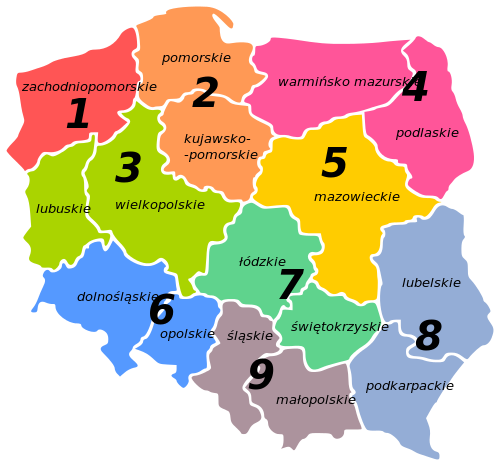
\includegraphics[width=150pt]{./Polish_HAM_Radio_Regions.png}
 \caption{Mapa okręgów wywoławczych w Polsce}
\end{figure}

\section{Co to są znaki okolicznościowe?}
Formalnie chodzi o pozwolenie dodatkowe. Są to znaki nadawane na okres maksymalnie jednego roku, np. dla uczczenia jakiegoś wydarzenia lub osiągnięcia. Znak dodatkowy uzyskuje się w UKE, tak jak każdy inny znak. Pozwolenie dodatkowe funkcjonuje równolegle z podstawowym - w trakcie pracy można korzystać zarówno z pozwolenia podstawowego jak i dodatkowego. Często w ramach pozwolenia dodatkowego krótkofalowcy posiadają znak używany podczas zawodów. 

\section{Czy mogę nadawać z mocą ,,ile fabryka dała''?}
Powinno się nadawać maksymalnie z mocą, która wystarcza do przeprowadzenia łączności, ale nie większą niż tą podaną w pozwoleniu. Przy większych mocach nie ma większego zysku, wiec nawet nie ma sensu marnować prądu na to, żeby wytracał się na antenie ;) Lepiej zrobić dobrą antenę niż sugerować się mocą nadajnika.
Łączność powinno się utrzymywać przy minimalnej mocy niezbędnej do komfortowej pracy. 

\section{Co to jest SWR i dlaczego warto zwracać nie niego uwagę?}
SWR to skrót od Standing Wave Ratio czyli po polsku Współczynnik Fali Stojącej (WFS). W dużym uproszczeniu, SWR mówi nam o niedopasowaniu impedancji nadajnika, linii zasilającej oraz anteny. Fala stojąca powstaje w linii zasilającej (kablu, fiderze zwał jak zwał), w wyniku niedopasowania impedancji falowej tejże linii do impedancji falowej anteny. Standardowo impedancja wynosi 50 Ohm, ale w wyniku różnych czynników takich jak np.: długość kabla, jakość złączy, jakość kabla impedancja linii zasilającej zmienia się. 

Niedopasowanie powoduje, że nie cała energia wypromieniowana do fidera z radiotelefonu jest dostarczona do anteny. Część energii odbija się i “wraca” do nadajnika co powoduje powstanie fali stojącej. Im wyższy SWR, tym więcej energii wraca do nadajnika a mniej energii jest wypromieniowane przez antenę. Energia wracająca do nadajnika powoduje nagrzewanie jego się stopnia wyjściowego, co przy dużym niedopasowaniu i długim nadawaniu może spowodować jego przegrzanie się i uszkodzenie.

W powyższych założeniach rozważaliśmy zmianę impedancji linii zasilającej, przy pracy nadajnika na częstotliwości rezonansowej anteny. Zmieniając częstotliwość nadawania, zmieniamy również impedancję anteny\footnote{\url{https://pl.wikipedia.org/wiki/Obwód_rezonansowy_LC}}.
Do pomiaru SWR używa się urządzeń zwanych reflektometrami\footnote{\url{https://pl.wikipedia.org/wiki/SWR_meter}}, lub o wiele bardziej zaawansowanych analizatorów antenowych.
Do prawidłowego pomiaru przydatne jest również sztuczne obciążenie. Dzięki niemu możemy najpierw przetestować linię zasilającą, następnie antenę na innym kablu, co pozwala nam ocenić czy problem wynika z uszkodzenia fidera (kabla linii zasilającej), anteny czy złącz.

Innym, nieco precyzyjniejszym parametrem opisującym to samo zjawisko jest Return Loss (RL) wyrażany w decybelach (dB).

\section{Dlaczego „jak nie wiesz co zrobić to zrób antenę”?}
Anteny można podzielić do dookólne i kierunkowe. Im bardziej kierunkowa jest antena, tym ma większy zysk, bo więcej mocy jest wykorzystane do promieniowania fal radiowych w konkretnym kierunku i więcej energii jest odbierane z tego kierunku. Na przykład dla anteny Yagi-Uda dodawanie elementów do anteny, zwiększa jej zysk energetyczny, a także kierunkowość.
Policzmy - różnica pomiędzy 100 W a 400 W, czyli czterokrotny zysk mocy, to czterokrotnie mocniejszy sygnał odbierany (+6dB), czyli tylko 1 punkt na S-metrze w radiu - 1S więcej.

Zamiast używać nadajnika o większej mocy, możemy niewielkim kosztem zrobić antenę, która będzie miała większy zysk energetyczny. Zysk energetyczny jest to stosunek mocy promieniowania w danym kierunku naszej anteny do mocy anteny wzorcowej, którą najczęściej jest dipol (półfalowy) (dBd) lub antena izotropowa (dBi). Zysk dipola jest większy w stosunku do anteny izotropowej o 2,15 dB więc: 0 dBd = 2,15 dBi. Antena z zyskiem 3 dBd w danym kierunku emituje 2 razy więcej energii w niż dipol. W zależności od rodzaju anteny, można osiągnąć zysk energetyczny od kilku do nawet kilkudziesięciu dBd. W ten sposób dostarczając do anteny taką samą energię, możemy wyemitować dużo silniejszy sygnał w określonym kierunku. Radiomatorzy zazwyczaj najpierw budują anteny kierunkowe na przynajmniej jedno pasmo, a dopiero później korzystają ze wzmacniaczy mocy.

\section{Czy radia muszą mieć atesty, certyfikaty, zaświadczenia, świadectwa dopuszczenia?}
Radioamatorzy jako jedyna grupa nadawców radiowych jest zwolniona z tego obowiązku. Dzięki temu możemy używać (a nawet powinniśmy) sprzętu - anten, nadajników, odbiorników własnej konstrukcji. Co bardziej ambitni mogą próbować używać naturalnych elementów otoczenia jako anteny. Znane są przypadki używania… karnisza jako anteny.

\section{Jaka antena jest najlepsza na początek?}
Najlepiej zaczynać z najprostszymi antenami, takimi jak prosty dipol półfalowy, pionowa ćwiartka (antena ćwierćfalowa), inverted vee (dipol w konfiguracji odwróconego V), a potem zabierać się za wielopasmowe anteny z trapami (filtrami LC odcinającymi sygnały powyżej danej częstotliwości), czy skomplikowanymi układami strojenia.

Na pasma krótkofalowe (szczególnie 80 m, 60 m, 40 m, 30 m i 20 m) najlepsze efekty osiągniemy przy antenach tzw. pełnowymiarowych, w których element promieniujący (pręt lub linka) będzie mieć wymiary niemal równe jedną czwartą długości fali. Wyjątkiem jest delta, która jest anteną o długości zbliżonej do jednej długości fali, przewodnik o tej długości jest ułożony w kształcie trójkąta. Reasumując - dipol jest jedną z najprostszych anten i jednocześnie jest całkiem skuteczna. Trudno zrobić antenę, która byłaby równie uniwersalna, prosta w budowie i skuteczna jednocześnie.

Jeśli chodzi o UKF, to na pierwszą antenę warto wybrać antenę możliwie dookólną, szczególnie jeśli nie wiemy w jakim kierunku są okoliczne stacje. Może to zaoszczędzić frustracji po półgodzinnym, bezskutecznym kręceniu anteną w poszukiwaniu upragnionego kontaktu. Anteny pionowe najczęściej są antenami dookólnymi, ale na niskie pasma mają dużą wysokość.

W antenę warto zainwestować również przy okazji prób używania prostych odbiorników typu SDR (np. RTL-SDR). Anteny dołączane do zestawu można traktować jako atrapy, nie dość, że są umieszczane blisko komputera, który jest dużym źródłem zakłóceń, to jeszcze są niedopasowane do interesujących nas częstotliwości.

Na pasma UKF-owe bardzo chwalone i polecane są Yagi autorstwa DK7ZB\footnote{\url{http://dk7zb.darc.de}} ,,krótkie'' wersje można zrobić tanio i w dodatku bez większego nakładu pracy.

\section{Co to jest ten KF/UKF?}
KF czyli fale krótkie to częstotliwości od 1 do 30 MHz.
UKF to pasma od 30 MHz do 1GHz. 
UKF można podzielić na VHF (ang. Very High Frequency) - w Polsce to 50, 70 i 144 MHz, UHF (ang. Ultra High Frequency), czyli fale decymetrowe (70, 23 i 13 cm) i SHF (ang. Super High Frequency), czyli mikrofale.

\section{Co z anteną, jeśli mieszkamy w bloku?}
Przed instalacją koniecznie należy poinformować administratora budynku. Zazwyczaj nie mają nic przeciwko temu, że na bloku sobie wisi jakiś drut. Za to czasami w domkach jednorodzinnych jest większy problem z powodu nadwrażliwych sąsiadów ;)
Jeśli mamy mieszkanie własnościowe to należy nam się dostęp do dachu. I nie ma, że boli, że dach na gwarancji. Należy się i już.
Do komina można montować maszt tylko za pomocą specjalnych opasek (bez ingerencji w strukturę komina). Maszt wraz z antenami nie powinien mieć więcej jak 3.0 m ponad poziom dachu (przepisy budowlane zezwalają na maszty do 3 metrów bez pozwolenia). Wyższe maszty powinny być wyposażone w odciągi oraz wymagają zgłoszenia w odpowiedniej instytucji.

\section{Czy metalowy balkon nie jest przypadkiem przeszkodą?}
Przy odpowiednim dystansowaniu anteny (więcej niż 1/4 fali od balkonu) nie będzie on przeszkadzał. Inaczej balkon robi za dodatkowy element anteny, który niekoniecznie musi nam pomagać.

\section{Jak zrobić najprostszą antenę?}
Najprostszą anteną jest dipol półfalowy. Wykonuje się go na konkretne pasmo w ten sposób, że liczy się długość fali i mnoży ją przez współczynnik skrócenia, zależny od grubości linki używanej do budowy dipola. Linkę dołącza się do przewodu koncentrycznego tak, że jedno ramię dipola dołączone jest do żyły środkowej, a drugie - do oplotu kabla. Tak połączony przewód rozwieszamy poziomo. Przykładowy dipol dla pasma 40 m ma dwa odcinki linki 1 mm\(^2\) o długości 9,5 m każdy. Dla pasma 20 m są dwa odcinki po 4,9 m każdy. Taki dipol będzie najlepiej pracował na początku pasma. Jeśli planujemy korzystać z anteny głównie w środkowym wycinku (tam, gdzie jest więcej łączności na SSB), antenę trzeba trochę skrócić, kierując się przy tym wskazaniami reflektometru (można wykorzystać wbudowany w większość fabrycznych transceiverów lub zewnętrzny) lub analizatora antenowego. Zbudowana w ten sposób antena, zawieszona nie niżej niż 5m nad ziemią, daje naprawdę spore możliwości. Dipol będzie pracować lepiej, jeśli zasilać go będziemy z użyciem symetryzatora (nazywanego skrótowcem balun od balanced-unbalanced, czyli symetryczny-asymetryczny), który umożliwi sprawniejsze przekazanie energii z kabla zasilającego do dipola, który jest anteną symetryczną.
Jest to tak prosta antena, że może być wykonana samodzielnie, z prawie dowolnych materiałów. Znamy przykłady dipoli wykonanych z linki do bielizny, która miała stalową żyłę w środku. Jeden z kolegów, jako żart, wykonał dipol na 40 m z drutu kolczastego. Ten niecodzienny materiał nie przeszkodził mu zrobić kilkuset łączności z innymi krajami w Europie.

\section{Czy dipol może działać na więcej niż jednym paśmie?}
Tak, ale nie zawsze. Dipol na pasmo 7 MHz może działać na paśmie 21 MHz (częstotliwość trzy razy większa), ale będzie się stroić nieco inaczej i nie zawsze umożliwi pracę na całym paśmie. Z kolei ten sam dipol na 7 MHz nie bardzo nadaje się do pracy na 14 MHz, gdyż ma tam bardzo wysoką impedancję, co wymaga szczególnego urządzenia dopasowującego. Aby wykonać dipol wielopasmowy, wykonuje się go jako tak zwany ,,fan dipol'', gdzie to samo zasilanie w.cz. (kabel plus ew. balun) zasila więcej niż jeden dipol, poszczególne elementy są rozwieszone w różnych kierunkach. Trzy dipole (80 m, 40 m, 20 m) połączone do wspólnego zasilania obsłużą cztery pasma (80 m, 40 m, 20 m, 15m). Jest to jedna z najtańszych i najprostszych anten wielopasmowych, możliwa do wykonania przez każdego. Wymaga nieco więcej miejsca od pojedynczego dipola, gdyż dla najsprawniejszego działania każdy z dipoli powinien wisieć w odstępie co najmniej kilku metrów od drugiego.

\section{Jakie jest minimalne wyposażenie stacji na KF?}
Transceiver przynajmniej na jedno pasmo (może być starszy, używany i popularny transceiver razem z niezbędnym wyposażeniem takim jak mikrofon), antena (może być dipol), kabel antenowy (na początek może być tani RG58) oraz źródło zasilania transceivera (najczęściej jest nim jakiś zasilacz o parametrach właściwych dla danego transceivera).

\section{Jaki jest koszt całej imprezy?}
W zależności od potrzeb. Można zacząć od zabawy w „nasłuchowca” kupując ,,RTL-SDR'' za kilkadziesiąt złotych, można zacząć od prostego radia ręcznego w okolicach 200 zł. Jeśli ktoś nie jest fanem łączności na fonii lub emisjami cyfrowymi, to można kupić dobre i wydajne radio jedno bądź kilkupasmowe za mniej niż 1000 zł. Z tzw. allbanderami (urządzenie obsługujące wszystkie podstawowe pasma amatorskie, zwykle z zakresu 160 m - 70 cm) sytuacja jest już troszkę mniej ,,kolorowa'', gdyż za nowy sprzęt trzeba czasami od 3 tysięcy złotych. Na szczęście w środowisku można znaleźć osoby, które sprzedają używany sprzęt za sensowne pieniądze.
Całość kosztów administracyjnych to: 50 zł opłaty za egzamin + 25 zł za wydanie świadectwa radiooperatora + 82 zł za wyrobienie i wydanie pozwolenia radiowego. I koszt dojazdów na egzamin, ewentualnego parkingu, czy przysłowiowego hot-doga na stacji paliw. Oraz znaczków pocztowych i koperty, ponieważ część dokumentów trzeba wysłać tradycyjną pocztą do UKE do Warszawy.

\section{Czy egzamin jest trudny?}
Nie, baza pytań jest ogólnodostępna, a większość odpowiedzi jest możliwa do wydedukowania. Pytania różnią się poziomem, ale większość z nich jest raczej ogólna niż szczegółowa.

\section{Gdzie można znaleźć pytania do egzaminu?}
Pytania do egzaminu można pobrać na stronie UKE\footnote{\url{bip.uke.gov.pl/download/gfx/bip/pl/defaultaktualnosci/125/20/18/materialy_pomocnicze_kategoria_1.pdf}}.
c
\section{Co to jest stacja automatyczna?}
Stacja automatyczna, to rodzaj radiostacji, do której obsługi nie jest potrzebny człowiek (najwyżej do nadzoru). Zazwyczaj są to przemienniki, bikony (ang. beacon), stacje meteorologiczne, balony różnej maści, czy eksperymenty. Taka stacja może dostać licencje kategorii piątej, znak zaczynający się prefiksem SR i maksymalną mocą nadawania poniżej 30 MHz - 50 W, a powyżej 10 W.
Stację automatyczną można uruchomić na okres testowy do trzech miesięcy pod własnym znakiem.

\section{Czym różni się pozwolenie radiowe od świadectwa radiooperatora?}
Ustawa z dnia 12 lipca 2024 r. - Prawo komunikacji elektronicznej zlikwidowała świadectwa i w ich miejsce wprowadziła zaświadczenie. Wcześniej wydane świadectwa nadal pozostają ważne.
Świadectwo radiooperatora świadczy o posiadaniu umiejętności w zakresie obsługi stacji radioamatorskiej, jest to dokument wydawany po zdanym egzaminie, nie uprawnia nas on jednak jeszcze do nadawania. Świadectwo jest wydawane dożywotnio i jest konieczne do uzyskania pozwolenia radiowego, dzięki któremu uzyskujemy możliwość nadawania na pasmach krótkofalarskich. Pozwolenie radiowe jest dokumentem uprawniającym nas do nadawania, wydawane jest zwykle na okres 10 lat, zawiera w szczególności nasz znak wywoławczy, lokalizację stacji i dane operatora.

\section{A jeśli zmieniam miejsce zamieszkania, to co?}
UKE bezpłatnie zmienia adres lub inne dane na pozwoleniu. Wystarczy np. poprzez system ePUAP wysłać wniosek o zmianę danych. 

\section{Jak uzyskać pozwolenie radiowe?}
Po pierwsze należy zapisać się na odpowiednią sesję egzaminacyjną, dokonać opłaty za egzamin. Po zdanym egzaminie należy wnieść opłatę za wydanie pozwolenia radiowego oraz udać się z wnioskiem o wydanie takiego do UKE\footnote{\url{bip.uke.gov.pl/jak-uzyskac-rezerwacje--pozwolenie--zezwolenie-tresc/pozwolenia-amatorskie,6,0.html}}. Na wniosku możemy we właściwych polach wskazać trzy proponowane znaki wywoławcze, w kolejności, w której chce się, żeby były rozpatrywane - przyznany zostanie pierwszy wolny spośród wskazanych. Następnie należy zaczekać na otrzymanie pozwolenia radiowego i od daty zawartej w pozwoleniu możemy w pełni legalnie działać na odpowiednich pasmach amatorskich.

\section{Czy mogę używać radia bez pozwolenia?}
Są wydzielone pasma, jak PMR, czy CB nie wymagające pozwolenia radiowego, ale są one regulowane innymi zasadami. Należy pamiętać, że nie są to pasma amatorskie i uzyskanie pozwolenia radiowego nie uprawnia nas do nadawania na nich z większą mocą, czy z własnoręcznie wykonanego sprzętu. Na pasmach amatorskich trzeba koniecznie posiadać pozwolenie do nadawania.

\section{Czym różnią się pasma amatorskie od PMR, CB i innych ogólnodostępnych?}
Radioamatorzy mogą nadawać z dużo większą mocą, z lepszego sprzętu. Zwykle mają znacznie lepsze anteny, mają do dyspozycji wycinki częstotliwości w praktycznie każdym fragmencie pasma.
Od doboru pasma zależy m.in. możliwy i oczekiwany zasięg naszej komunikacji. Pasma PMR i CB to pasma jedynie z ograniczeniem klasy (w tym mocy i generalnie parametrów) sprzętu. Praktycznie nie działają tam zasady radiooperatorskie, często można też doświadczyć dużo niższego poziomu prowadzonych rozmów, czy braku wzajemnego szacunku między operatorami. Zaletą pasm ogólnodostępnych jest głównie brak konieczności posiadania pozwolenia radiowego do korzystania z nich.

\section{Co to jest klub radioamatorski?}
Klub krótkofalarski, jest to jak nazwa wskazuje, organizacja skupiająca krótkofalowców. Są to stacje, gdzie operatorem może być każdy (oczywiście pod nadzorem operatora klubowego). Kluby często posiadają specjalistyczny sprzęt pomiarowy, wyczynowe anteny, czy bardziej zaawansowane radia. Klubowicze często pomagają sobie wzajemnie m.in. przy budowaniu nadajników, anten, przy regulacji sprzętu, wykonują wzajemne łączności. 

\section{Jakie są zasięgi sprzętu amatorskiego?}
Samo słowo “zasięg sprzętu” jest trochę niefortunnym określeniem, gdyż samo to “gdzie się dociera” zależy od wielu czynników, takich jak pogoda, warunki propagacyjne, pora dnia, moc nadajnika, skuteczność modulacji, zysk anteny i wiele innych czynników. Nawet takie niby niepozorne rzeczy, jak promieniowanie słoneczne, czy mgła mogą znacząco wpłynąć na poprawę lub pogorszenie “zasięgu”.
Na dodatek zawsze w łączności są dwie stacje. To, że z domowej anteny z mocą 50 W da się zrobić łączność z kimś z Tarnowa, kto ma również dobrą antenę nie znaczy, że da się taką samą łączność zrobić z kimś kto ma ręczniaka z małą antenką. 
\\

Dla bardzo wielkiego uproszczenia (mówimy oczywiście o UKF-ie):\\
ręczniak $\Leftrightarrow$ ręczniak 1 - 10 km\\
ręczniak $\Leftrightarrow$ baza 5 - 30 km\\
samochód $\Leftrightarrow$ samochód 10 - 30 km\\
baza $\Leftrightarrow$ baza 50 - 150 km \\

W optymalnych warunkach przemiennik może zwiększyć ten zasięg dwukrotnie.
W wypadku podniesionych warunków propagacyjnych da się przeprowadzić łączności Krakowa z Warszawą albo usłyszeć stacje np. z Kaliningradu.
Na falach krótkich (1,8-30 MHz) zasięgi łączności wahają się od kilkuset kilometrów do całego świata. 
Dużo zalezy też od samych umiejętności operatora, poziomu zakłóceń itp. 

\section{O co chodzi z „warunkami” na pasmach?}
Jonosfera nie zachowuje się cały czas tak samo. Czasem fala odbija się lepiej innym razem gorzej. Czasem tłumienie trasy czyli strata sygnału po drodze jest większa a czasem mniejsza. 
Sporo zależy też od aktywności słońca.

\section{Jak zacząć przygodę z nasłuchem czyli RTLSDR?}
Historia RTLSDR wygląda mniej więcej tak: podczas pisania linuksowego sterownika dla układu rtl28832 i podobnych okazało się, że moduł ten udostępnia znacznie więcej danych z odbiornika niż można by oczekiwać od odbiornika telewizji naziemnej. Napisano więc „sterownik” (nie jest to sterownik ładowany do jądra, ale specjalny w user space, wykorzystujący bibliotekę libusb), który potrafi odebrać i zinterpretować dane z niego. W ten sposób uzyskano bardzo tani odbiornik „SDR” (Software Defined Radio).

Główną zaletą tego typu odbiorników jest to, że całość demodulacji wykonujemy programowo. Jeśli nagle chcemy odebrać coś w modulacji AM - nie ma problemu. Chcemy posłuchać SSB? Nie ma problemu. Chcemy zobaczyć jakie dane wysyła nasz licznik wody czy pilot od bramy garażowej? Nie ma problemu - wystarczy tylko odpowiedni kawałek oprogramowania.

Na początek przygody z RTLSDR bardzo polecamy zapoznanie się z systemem ADS-B używanym w lotnictwie. Istnieją bardzo dobre programy umożliwiające demodulację tych sygnałów, w dodatku nadajniki są bardzo korzystnie rozlokowane (w samolotach), więc wystarczy nam dość prosta antena aby odbierać sygnały z obszaru wielu kilometrów! Na początek jest to bardzo satysfakcjonujące zajęcie.
Ważną rzeczą przy korzystaniu z RTLSDR jest pamiętanie o używaniu odpowiednich anten. Atrapy anten dołączane do zestawu zwykle średnio nadają się nawet do drapania za uchem, a co dopiero do odbierania jakichkolwiek sensownych sygnałów. Nawet najprostszy kawałek drutu (KD) uformowany w tzw. dipol półfalowy (brzmi groźnie, ale to naprawdę jest kawałek drutu) pozwoli nam na dużo szybsze odnalezienie sygnałów w otaczającym paśmie.
Trzeba również pamiętać o tym, że odbiorniki te lepiej odbierają na UKFie, a na KFie trzeba uruchomić tryb ,,direct sampling'', który umożliwia odsłuch poniżej 25 MHz.
Według przysłowia ,,biedny dwa razy traci'' nie należy też kupować najtańszego takiego odbiornika, bo szybko rozczarujemy się jego niewielkimi możliwościami. Najlepiej zapytać bardziej doświadczonych kolegów lub koleżanki.
Można polecić ten oferowany na stronie rtl-sdr.com. 

Drugą ważną rzeczą jest to, że te odbiorniki zwykle charakteryzują się stosunkowo małą czułością i sytuacje, kiedy sprzęt klasy amatorskiej odbiera daną transmisję bardzo dobrze, zaś RTLSDR ledwo „łapie” są niestety dość częste. Na szczęście można kupić odbiorniki (czy nawet nadajniki) SDR charakteryzujące się bardzo dobrymi parametrami - są nawet projekty używające tego typu urządzeń do tworzenia własnych sieci GSM!

Techniczne aspekty używania SDR-ów zasługują na osobny artykuł, więc żeby nie przedłużać wspomnimy tylko o kilku najważniejszych rzeczach: silny sygnał pojawiający się na środku analizowanego wycinka pasma to niestety, zwykle szum własny odbiornika, nie należy liczyć na „czysty” odbiór w jego okolicy - lepiej dostroić się do częstotliwości gdzieś obok, a później tylko wyciąć interesujący nas kawałek. Warto wspomnieć o słabej, fabrycznej kalibracji odbiorników RTLSDR. Kalibrację jednak można wykonać bardzo łatwo (m.in. do znanych częstotliwości nadajników GSM).
Z nazewnictwa „wodospad” to „wykres widma w czasie”, a tłumacząc „z polskiego na nasze” to rysunek, na którym możemy zobaczyć (zwykle silniejszym, zbliżającym do czerwieni, kolorem) na jakiej częstotliwości pojawiały się w ciągu ostatnich kilkudziesięciu sekund sygnały.

\section{Czy mogę nasłuchiwać bez użycia RTLSDR?}
Odbiorniki bez nadawania to tzw. skanery. Wszelkiej maści urządzenia które są jedynie odbiornikami można używać bez większych ograniczeń. Nie wolno używać urządzeń posiadających możliwość nadawania bez pozwolenia. Oczywiście temat „czy można słuchać służb” i innych pasm nieprzeznaczonych dla cywili zasługuje na osobne rozważania, które poruszamy w innym pytaniu.

\section{Co to jest WebSDR, czy mogę go użyć i jak to zrobić?}
WebSDR\footnote{\url{http://websdr.org/}} to technologia dzięki której można udostępnić swój odbiornik SDR wielu użytkownikom, zwykle przez Internet. Ciekawostką jest to że z jednego odbiornika może korzystać wielu użytkowników w ten sposób, że każdy z nich słucha innej częstotliwości. Dzieje się tak ponieważ odbiorniki SDR zwykle są w stanie słuchać na tyle szerokiego pasma, że zawiera ono w sobie wiele kanałów komunikacyjnych, a każdy z użytkowników może „dostroić” się do interesującego go wsygnału na określonym wycinku pasma, czy pojedynczego kanału z interesującą go modulacją. W odnośniku na dole strony można znaleźć listę serwerów WebSDR. W Polsce serwery znajdują się w Zielonej Górze\footnote{\url{http://websdr.sp3pgx.uz.zgora.pl:8901/}} i w Dubiecku, ten drugi jest jednak w chwili obecnej wyłączony.


\section{Gdzie znaleźć rozszyfrowane skróty używane przez radioamatorów?}
Skróty kodu Q i slang można znaleźć w artykule na Wikipedii\footnote{\url{http://pl.wikipedia.org/wiki/Kod_Q}}, całej reszty można się nauczyć słuchając, czy po prostu pytając. Krótkofalowcy to naprawdę mili ludzie. Ewentualnie możemy posiłkować się oficjalnymi dokumentami pierwszego regionu IARU nazwanego “HF Manager Handbook” w wersji najnowszej - można go zawsze znaleźć na stronach IARU\footnote{\url{http://www.iaru-r1.org/}}.

\section{Na jakich częstotliwościach najszybciej znajdę inne stacje i najlepiej zacząć wywołanie?}
A na jakie pasmo masz radio?
Jeśli na 2 m to zacznij od 145,550 MHz, to taka trochę krakowska częstotliwość wywoławcza. Wołają tam też stacje z gór (m.in. w programie SOTA) (głównie w lecie). Na częstotliwości 145,500 MHz są zwykle łączności typu DIRECT czyli bezpośrednie pomiędzy stacjami. Jeśli masz zdrowie do słuchania gadania o niczym to polecamy okoliczne przemienniki.

\section{Co to jest AM, FM, CW, SSB, USB, LSB?}
\begin{itemize}
\item AM to modulacja amplitudy - do częstotliwości nośnej dodawana jest częstotliwość sygnału modulowanego. 
\item LSB i USB to modulacje jednowstęgowe (SSB) są tworzone przez tłumienie fali nośnej i odpowiedniej dla danej modulacji wstęgi bocznej. 
\item FM to modulacja, gdzie wraz z amplitudą sygnału zmienia się częstotliwość nadawanego sygnału. 
\item CW to przerywanie (kluczowanie) fali nośnej, którym nadaje się alfabetem Morse'a, czyli telegrafią. \end{itemize}

\section{Jak to jest z telegrafią?}
Jest to najstarsza emisja. Polega ona na załączaniu i wyłączaniu fali nośnej w takt sygnałów alfabetu Morse'a. Jeszcze dwadzieścia lat temu była wymagana na egzaminie, by móc nadawać na falach krótkich. Obecnie nie jest wymagana, ale mimo to sporo radioamatorów się jej uczy. Jest sprawna energetycznie oraz skuteczna podczas silnych zakłóceń, nadajnik może być bardzo prosty, ale wymaga umiejętności operatora. Trzeba umieć odbierać sygnały telegraficzne, by sprawnie posługiwać się tą emisją. Proces nauki jest dość żmudny, ale doświadczenia kolegów z grupy Titawa\footnote{\url{http://titawa.pl}} pokazują, że nowoczesne metody nauki są skuteczne. Istnieją programowe dekodery telegrafii, ale ich sprawność jest ograniczona, popełniają dość dużo błędów. Człowiek nadal jest lepszy. Wprawni telegrafiści mogą rozmawiać prawie tak samo, jak na fonii, tylko trochę wolniej. Doświadczenia kolegów pokazują, że przy dobrej motywacji i chęci, telegrafii można się nauczyć w trzy-cztery miesiące codziennych ćwiczeń i po takiej nauce z powodzeniem robić łączności z innymi krótkofalowcami, a nawet startować w zawodach.

\section{Czy nauka telegrafii jest trudna?}
Nie! Wiele osób demonizuje naukę telegrafii popierając to argumentem własnej porażki, lub zupełnie niepopartymi naukowo, jak obowiązek posiadania ,,słuchu muzycznego''. Problemem jest jedynie odpowiednie podejście do tematu, zdefiniowanie celu, podzielenie go na mniejsze i ich skrupulatna realizacja. Nauka samej telegrafii polega na nauczeniu naszej głowy pewnych wzorców, które następnie nasz mózg podświadomie rozpozna. Wzorce te często nazywane są ,,melodią znaku'' i stąd analogia do umuzykalnienia i nieszczęsne przekonanie o konieczności posiadania muzycznych umiejętności, które wcale nie są wymagane, lecz oczywiście mogą pomóc w procesie nauki. Sama nauka bardziej zbliżona jest do nauki mowy, gdzie na początek uczymy się literek, następnie zaczynamy składać sylaby, pojedyncze słowa, a dopiero na sam koniec konstrukcje złożone w postaci logicznych zdań. Przez analogię w telegrafii uczymy się na początek literek, krótkofalarskich skrótów, kodu Q, a dopiero na koniec pracy otwartym tekstem. Tak samo jak mowy, tak i telegrafii nie nauczymy się w dwa dni, jest to proces długotrwały i żmudny, a przez to wielu wydaje się nudny i nieatrakcyjny, przez co porzucają naukę czasem nawet tuż przed metą. Przy odrobinie dodatkowej wiedzy o pułapkach naszego umysłu, dodaniu elementów zabawy i systematyczności, nauka ta ,,przyjdzie sama'' bez względu na to czym się zajmujesz i jakie masz talenty. W końcu przecież wszyscy posługujemy się mową, a telegrafia to trochę jak kolejny język, choć zdecydowanie łatwiej się jej nauczyć. 

\section{Na czym polegają zawody?}
Zawody radiowe najczęściej polegają na tym, aby zawodnicy nawiązali jak najwięcej łączności, najlepiej na jak największe odległości. Podczas zawodów na falach krótkich najczęściej osobno są przyznawane punkty za stacje lokalne, czyli z tego samego kontynentu, a większa liczba punktów jest przyznawana za stacje DX, czyli znajdujące się na innym kontynencie. Podczas zawodów UKF bardzo często liczy się każdy kilometr łączności. Regulaminy zawodów czasami zawierają ciekawe zapisy utrudniające pracę, które powodują, że zawody są ciekawsze.

\section{Co oznacza ,,UP 5''?}
UP 5 oznacza, że korespondent pracuje w tzw. splicie (ang. split), czyli nadaje i słucha na różnych częstotliwościach oddalonych od siebie np. o 5kHz. Jeśli takiego korespondenta słyszymy np. na częstotliwości 14,303 MHz to oznacza, że my powinniśmy nadawać na częstotliwości 14,308 MHz. Split pozwala łatwiej ogarnąć dużą liczbę korespondentów. 

\section{Co to są transmisje cyfrowe i jak bardzo mam się tym przejmować?}
To zależy czy cyfrówki Cię wciągną. 
Jest cała masa różnych rodzajów transmisji cyfrowych. Jest RTTY i PSK31 i trzeba wspomnieć że zwłaszcza PSK jest diablo skuteczna. To czego się nie zaliczy na fonii, cyfrowo wpada z niezłymi raportami. Ostatnio dużą popularnością cieszy się FT8.
Jak masz ciśnienie na zaliczanie podmiotów DXCC albo żonę która ma już dość szumu w domu, to cyfrówki są alternatywą.

Jeśli chcesz ,,zrobić'' Japonię, lub inny dalszy kraj małą mocą, to warto zainteresować się JT65 lub FT8 - bardzo skuteczne rozwiązania. Na KF-ie jest sporo miłośników emisji cyfrowych - jest to w sumie jedyna możliwość, jeśli interesuje kogoś pasmo 30 m, a z telegrafii słabo mu idzie. Poza tym są stałe częstotliwości - 7040-7050, 14076-14090, 18100-18105, 21076-21090 i tak dalej - wszystko jest do znalezienia w bandplanie regionu 1 IARU.

Trochę osobną kategorią są emisje cyfrowe w pasmach UKF, gdzie bardzo często wykorzystuje się zmodyfikowane emisje wprost z łączności profesjonalnej jak DMR. Jest też C4FM,DSTAR czy Fusion. Jeśli masz radio SSB to spotkasz też transmisje jak na KF i wiele innych specjalistycznych dedykowanych do łączności w tzw. "sporadycznych warunkach". 

Do transmisji cyfrowych używać będziesz częściej komputera niż mikrofonu, a uzyskiwane zasięgi łączności z pewnością nie raz Cię zaskoczą. Musisz być cierpliwy i monitorować warunki bo następna 'okazja' do dalekiej łączności może być dopiero za wiele tygodni

\section{Co to jest podmiot DXCC?}
Amerykański związek krótkofalowców (ARRL\footnote{\url{www.arrl.org}}) wydaje dyplom DX Century Club (DXCC). W dyplomie tym licza się kraje i podmioty w rozumieniu krótkofalarskim. Każda dyskretna jednostka geograficzna lub polityczna jest uważana za kraj. Np Alaska czy Hawaje sa zaliczane jako osobny podmiot, pomimo przynależności do USA. ARLL publikuje listę\footnote{\url{http://www.arrl.org/files/file/DXCC/2022_March_DXCC_Current.pdf}} takich podmiotów DXCC.

\section{Czy przez radio mogę wysyłać dane i jeśli tak to jak?}
Oczywiście. Istnieje ,,Packet Radio'', czyli łączności z wykorzystaniem protokołu AX.25, stosowane raczej na pasmach UKF-owych do przesyłania krótkich paczek danych, podobnie jak w Internecie.
Jest APRS.
Jest też PSKmail oraz Winlink.
Istnieje także HAMNet, który w Polsce powoli zaczyna powstawać\footnote{\url{http://hamnet.pl}}.

\section{Co to jest APRS?}
APRS czyli automatyczny system raportowania pozycji to system pozwalający na informowanie o bieżącym położeniu stacji amatorskich. W wysyłanej ramce można zamieścić krótki opis, położenie oraz typ stacji (stała, ruchoma, przenośna itd). Wykorzystywany jest głównie w samochodach choć nie tylko. Poza standardowymi stacjami na APRS-ie można też znaleźć dodatkowe punkty informujące o lokalnych przemiennikach, stacje pogodowe wraz z danymi z tych stacji, telemetrię balonów meteorologicznych, informacje o zagrożeniach itd. 
Poza tym przy pomocy APRS-u można wysyłać sobie wiadomości podobne do SMS-ów.
Całość oparta jest o protokół AX.25 i działa zazwyczaj na częstotliwości 144,800 MHz. Istnieją częstotliwości APRS na innych pasmach, w tym również w paśmie 70 cm.
Do działania potrzebne jest zwykłe radio FM na pasmo 2 m oraz modem, np. typu TNC lub tracker. 
Pewną namiastką jest program na Androida o nazwie APRSdroid, który potrafi korzystać z APRS-u po TCP/IP lub odbierać i generować ramki audio.
Dane z APRS-u można oglądać w internecie na stronie aprs.fi

\section{A o co chodzi z tymi satelitami?}
Istnieje wiele satelitów, które posiadają przemienniki liniowe lub FM. Można przez nie nawiązywać łączności z zachowaniem odpowiednich norm (nadawanie małą mocą, wąska modulacja itp.). W łącznościach przez satelity specjalizuje się część radioamatorów, ale część korzysta z nich w takim samym zakresie jak z łączności bezpośrednich lub przez przemienniki naziemne. Większość z satelitów stale się porusza i są ,,w zasięgu'' tylko przez chwilę, ale jest jeden satelita, a w zasadzie transponder amatorski QO-100 na pokładzie satelity geostacjonarnego Es'hail-2 (tak, tak taki do TV-SAT), przez który możesz robić łączności niewielkim zestawem nadawczo-odbiorczym i anteną na balkonie. W ,,zasięgu'' satelity są Europa, Brazylia, RPA czy Indie.

\section{Co to jest EME?}
EME (Earth-Moon-Earth), to łączności polegające na odbijaniu sygnału od powierzchni księżyca. Wymagają one rozbudowanych anten o znacznym zysku (długie Yagi) i dużych mocy, by można było chociaż ułamek mocy usłyszeć znów na Ziemi. Używa się do tego zazwyczaj wolnej telegrafii i transmisji cyfrowych (JT-65).

\section{O czym nie należy rozmawiać na radiu a co jest mile widziane?}
Zdecydowanie odpada polityka i religia. Chodzi po prostu o nie wywoływanie niepotrzebnych ideologicznych dyskusji. Trollowanie nie jest mile widziane, więc jeśli zaczniesz trollować i wyrobisz sobie opinię trolla, to po prostu ludzie zaczną Cię ignorować.
Skoro jest to służba radioamatorska, to powinno się rozmawiać właśnie na takowe tematy - sprzęt, łączności itp. Oczywiście nie są zabronione dyskusje na tematy ogólne - powinno się pomijać tematy delikatne, tabu i obraźliwe - kultura osobista również jest wskazana. Nie każdy chce dowiedzieć się o Twoich problemach zdrowotnych, czy preferowanej opcji politycznej.

\section{Co to jest grupa i jak należy „wymieniać się mikrofonem”}
Każdorazowo na zakończenie swojej relacji powinniśmy podać znak korespondenta i swój. Tak jest teoretycznie. Często traktujemy to mniej restrykcyjnie, ale kiedy rozmawia na jednej częstotliwości kilka osób przekazywanie mikrofonu staje się koniecznością. Chodzi o to, żeby pozostali wiedzieli kto teraz może się odezwać, bo inaczej powstają konflikty co kończy się wymiksowaniem sygnałów w niezrozumiały bełkot. Słowo „grupa” w takim wypadku jest sygnałem dla słuchających, że jest większe grono rozmówców niż tylko stacje, których znaki zostały wymienione.

Ważnym argumentem za podawaniem znaków (zarówna na KF jak i UKF) jest fakt, że w trakcie dłuższej pracy w grupie może pojawić się nowy słuchacz, który chce wiedzieć kto rozmawia. Może to być nadawca lub nasłuchowiec, który nie ma możliwości zapisania pełnego nasłuchu nie znając znaków.

\section{Co to jest łączność kryzysowa, EmCom? Dlaczego krótkofalarstwo to „służba” i jak powinniśmy wykorzystywać radia w sytuacjach kryzysowych?}
W przypadku wystąpienia nagłego bądź długotrwałego zdarzenia kryzysowego, radioamatorzy mogą okazać się jedynym środkiem, dzięki któremu najbliższe sąsiedztwo, lokalna społeczność będą w stanie przekazać informacje np. o potrzebie pilnej pomocy medycznej, pożarze, czy innej sytuacji, która wymaga interwencji służb ustawowo powołanych do niesienia pomocy. W takich sytuacjach, radioamatorzy stanowią alternatywne do łączności profesjonalnej tych służb, medium przekazu informacji. W czasie, gdy pozostali obywatele mogą być pozbawieni kontaktu, radioamatorzy są w stanie zapewnić łączność nawet wtedy, gdy na skutek zdarzeń kryzysowych uszkodzeniu ulegną komercyjne systemy telekomunikacyjne, takie jak telefonia stacjonarna, komórkowa czy Internet. Więcej informacji można znaleźć na stronie EmCom Polskiego Związku Krótkofalowców\footnote{\url{https://emcom.pzk.org.pl/}}.

W Polsce radioamatorzy ćwiczą scenariusze sytuacji kryzysowych organizowane przez SP EmCom, komórkę organizacyjną ds. łączności kryzysowej PZK. Najbardziej znana jest Dolnośląska Amatorska Sieć Ratunkowa, która okazała się w wielu miejscach jedynym środkiem łączności ze światem podczas powodzi w 1997 r.

\section{Czy i gdzie mogę posłuchać prognozy pogody?}
W Krakowie na częstotliwości 144,950 nadaje stacja pogodowa SR9WXR w modulacji FM. Jest ona w pełni automatyczna i co 15 minut nadaje pełne raporty pogodowe z takimi danymi jak zachmurzenie, temperatura, ciśnienie, wilgotność, prędkość wiatru, itd. Dodatkowo, stacja podaje również informacje o jakości powietrza w regionie oraz o warunkach propagacyjnych na różnych pasmach radiowych.

Stacja ta jak i wiele innych pogodowych stacji automatycznych używa ujednoliconego oprogramowania SR0WX\footnote{\url{https://github.com/sq9atk/sr0wx}} i jeśli nie jesteś z Krakowa, jest bardzo możliwe że w Twoim regionie również nadaje taka sama stacja, prawdopodobnie na podobnej częstotliwości.

Warto tutaj zaznaczyć, że sporo radiotelefonów - zazwyczaj ręcznych - ma w swoim menu opcję w rodzaju ,,weather alert'' lub ,,wx alert''. Działa to na takiej zasadzie, że radio albo wykorzystuje swój drugi odbiornik (jeśli taki ma), albo co jakiś czas przy braku odbieranych transmisji przełącza się na określoną w ustawieniach częstotliwość by sprawdzić, czy nie nadawany jest komunikat pogodowy. Jednakże, ta funkcja jest przystosowana w większości przypadków tylko do sytuacji w których przed raportem pogodowym nadawany jest na częstotliwości specjalny sygnał który nakazuje odbiornikowi nasłuchiwać dana stację. Taki sygnał nadają głównie profesjonalne stacje pogodowe, na przykład działające w ramach amerykańskiego NOAA. W Polsce ten standard nie jest generalnie wykorzystywany, wobec czego funkcja ,,wx alert'' nie zadziała z naszymi stacjami SR0WX lub podobnymi.

Pogodę można sprawdzić również po APRS-ie, większość radiotelefonów z obsługą tego systemu ma w swoim interfejsie ustawienia dot. przyjmowania informacji pogodowych.

\section{Czy można słuchać samolotów?}
Można. Mało to ciekawe na dłuższą metę, ale można.

\section{Czy można słuchać służb mundurowych?}
Technicznie słuchać można wszystkiego. Za to informacji zasłyszanych na pasmach innych niż amatorskie/ogólnodostępne nie wolno rozpowszechniać ani wykorzystywać. Jeśli transmisja jest szyfrowana nie wolno jej odszyfrowywać.

\section{Czy mając licencję będę mógł postawić własnego BTS-a lub wskrzesić pagery?}
Generalnie nie można uruchamiać typowych nadajników GSM, czy stacji bazowych dla pagerów na pasmach krótkofalarskich, ale da się stworzyć analogiczne urządzenia dopasowane do zasad i częstotliwości panujących na pasmach amatorskich. Przede wszystkim należy pamiętać o konieczności identyfikacji znakiem wywoławczym oraz o tym, że taka sieć/system będzie mogła być używana jedynie niekomercyjnie i tylko przez krótkofalowców. Oczywiście doświadczenie w pracy na pasmach amatorskich może później przydać się przy pracy przy komercyjnych systemach. 

\section{Gdzie można znaleźć więcej źródeł informacji o służbie radioamatorskiej?}
Znakomitym źródłem informacji są publikacje amerykańskiego ARRL\footnote{\url{http://www.arrl.org}} z serii ,,Handbook''. Znakomitymi publikacjami w języku polskim są zeszyty w opracowaniu Krzysztofa OE1KDA\footnote{\url{https://hf5l.pl/pdfs/}}. Polecamy też polskie\footnote{\url{http://sp-hm.pl/}} fora dla konstruktorów. Istnieje też nasza grupa ,,radiowa'' w komunikatorze Telegram\footnote{\url{https://t.me/+b7BuP-ZQUYxlNjJk}}. Można także osobiście wołać autorów tego dokumentu.

\end{document}
